\documentclass[tikz,border=3pt]{standalone}
\usepackage[utf8]{inputenc}
\usepackage[T1]{fontenc}
\usepackage{lmodern}
\renewcommand{\familydefault}{\sfdefault}
\usepackage{sansmath}\sansmath
\usepackage{chemfig}
\usepackage{pgfplots}\pgfplotsset{compat=1.18,/pgf/number format/use comma,/pgf/number format/1000 sep={.}}
\usetikzlibrary{arrows.meta,calc,positioning,decorations.pathmorphing,patterns}
% paleta del sitio
\definecolor{nar}{HTML}{E8680C}\definecolor{narc}{HTML}{FFB35C}\definecolor{hielo}{HTML}{FFF3E8}
\definecolor{tinta}{HTML}{1D1D1F}\definecolor{gris}{HTML}{6E6E73}\definecolor{lila}{HTML}{7C5CF0}
\definecolor{azul}{HTML}{2F6FD6}\definecolor{menta}{HTML}{17A673}\definecolor{coral}{HTML}{E8342A}
\begin{document}
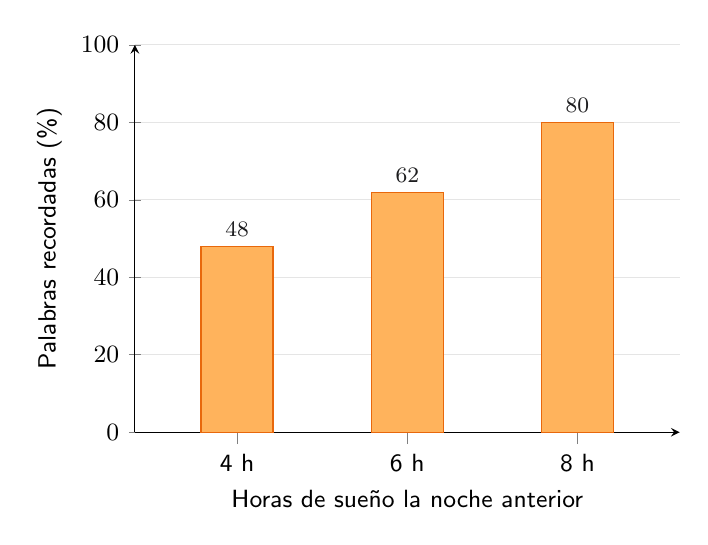
\begin{tikzpicture}[font=\small]
\begin{axis}[axis lines=left,ymajorgrids,grid style={gray!20},ybar,bar width=26pt,
  xlabel={Horas de sueño la noche anterior},ylabel={Palabras recordadas (\%)},
  width=8.5cm,height=6.5cm,xmin=0.4,xmax=3.6,ymin=0,ymax=100,xtick={1,2,3},xticklabels={4 h,6 h,8 h},ytick={0,20,...,100},
  nodes near coords,nodes near coords style={font=\footnotesize,text=tinta}]
\addplot[fill=narc,draw=nar] coordinates {(1,48)(2,62)(3,80)};
\end{axis}
\end{tikzpicture}
\end{document}
